%!TEX root = ../template.tex
%%%%%%%%%%%%%%%%%%%%%%%%%%%%%%%%%%%%%%%%%%%%%%%%%%%%%%%%%%%%%%%%%%%%
%% chapter2.tex
%% NOVA thesis document file
%%
%% Chapter with the template manual
%%%%%%%%%%%%%%%%%%%%%%%%%%%%%%%%%%%%%%%%%%%%%%%%%%%%%%%%%%%%%%%%%%%%
\chapter{Estado-da-arte}
\label{cha:stateOfTheArt}
%{\LARGE \textbf{~\\These instructions are outdated! Please see also the “template.tex” file!\\}}
%
%This chapter describes how to use the \LaTeX\ \novathesis\ template (and the “\novathesisclass” class file).
%
%Let's start with some simple suggestions:
%
%\begin{enumerate}
%  \item No! You don't have to use this template to write your thesis.  You don't even have to use \LaTeX.  However, writing a thesis is serious stuff, and which tool you shall use to write it is not a decision to make lighthearted.
%  \item \LaTeX\ is hard enough by itself.  This template aims at making your life easier, but not easy. If you choose to use this template to write your thesis, you are very welcome.  However, don't expect me to provide you help with \LaTeX.  Look for help with your friends (you have some friends, don't you?), or search the web, or try even to read some book(s) on \LaTeX. In the end you will certainly find the experience rewarding.
%  \item So, don't forget, when you come to the point of “\emph{How do I do this with \LaTeX?}” look for help!  Google is your best friend. 
%  \item If you believe the difficulty is related with the \novathesis\ template itself (and not with \LaTeX), please \textbf{do not} send me an email asking for help.  Please look for help in the \novathesis\ Google Group (URL) and the \novathesis\ Facebook group (URL).  If you can't find help there from previous posts/messages, then post your own question. Hopefully someone will answer you.
%\end{enumerate}
%
%Now, let's go to a major issue for Windows users.  Characters have to be encoded in files as numbers, and that is how character encodings were born. ASCII and EBCDIC standards are long lost in the past.  The world now uses UTF-8.  Well, not all the world… Windows is still stick in its \emph{codepages}, and “latin1” is what windows uses as the codepage for Western Europe. This messes up with the template. Please be sure you use an editor with UTF-8 support.  \emph{Go to the preferences/options/… of your text editor and set up its default file encoding as UTF-8.}

% section introduction (end)
\section{Docking}
\subsection{Modelos de docagem em relação à rigidez da superficie}
\label{classi}
Com o passar do tempo cada vez mais algoritmos e respetivas adaptações para simular a docagem dos complexos de proteinas têm surgido, adoptando modelos que formulam hipóteses em relação às caracteristicas dos elementos envolventes. 

Um algoritmo pode ser classificado em função da forma que trata a rigidez  da superficie dos pares de proteinas a juntar ou até mesmo pelo modelo matemático que os algoritmos seguem, como por exemplo se aplicam a Fast Fourier Transform ou não.

Serão abordadas nas próximas subsecções 3 modelos de docagem: flexivel, semi-flexivel e rigida. 

%Estes três conceitos são necessários para que se possa entender melhor os algoritmos nas secções seguintes, já que as suas complexidades dependem em certa forma da maneira como tratam a flexibilidade dos pares de proteinas e por consequência do número de dimensões que o espaço solução irá ter assim como a qualidade do conjunto solução encontrado.


	\subsubsection{Docagem Flexivel} Em que ambos os complexos receptor e ligando são considerados como sendo corpos flexiveis e adaptáveis sendo, no entanto, a mesma flexibidade interpretada pelo algoritmo de forma simplificada ou limitada, e por consequência pode-se aplicar um modelo através de simulações de docagem.

	\subsubsection{Docagem Semi-Flexivel} Um dos corpos é considerado rigido e o outro não, em situações normais este tipo de algoritmos trata o ligando como se fosse a proteina flexivel, já que este é mais pequeno do que o receptor, tendo assim uma maior probabilidade de mudar a sua forma, outra justificação tem a ver com os custos de computação serem mais baixos do que se considerarmos os receptores como flexiveis.

	\subsubsection{Docagem Rigida} 
	O par é considerado como sendo rigido na sua integridade, sendo também considerado que na docagem entre os dois corpos uma das proteinas irá acabar por penetrar a outra o que leva a que se tenha de adaptar o conjunto de soluções para o problema em seis 		dimensões de liberdade, 3 para a rotação e 3 para a translação. %cite 

Apesar de se considerarem as superficies de ambos como rigidos, considera-se que ocorrem variações na superficie permitindo que haja penetrações inter-moleculares.

Este modelo tem a vantagem a ser o mais rápido dos 3 a considerar, sendo capaz de explorar as superficies de ambos os elementos e traduzir para uma base de dados de docagem \cite{halperin}.


\subsection{Dinamica molecular}



\subsection{Fast Fourier Transform}
Algoritmo baseado em previsões geométricas sobre o complexo formado após a interação entre as proteinas, representando o método a partir do qual ocorreram adaptações que levaram origem à criação do BiGGER \cite{biggerPaper}.
É utilizado em muitos softwares especificos para \textit{protein docking} ( FTDock, 3D-Dock,GRAMM, ZDOCK,..)\cite{geometry}. 

A origem deste método remonta ao artigo de Katchalski Katzir et al \cite{katchalski1992} onde se considera que ambos os pares são corpos rigidos, o que no âmbito do ponto \ref{classi} pode-se assumir como docagem rigida. 

 À semelhança do BiGGER, este método também recorre a uma estimativa da complementaridade entre as superficies dos pares que compõem a PPI, apenas existe como requisito o conhecimento da estrutura tri-dimensional destes.
 
 A metodologia com que são determinadas as possibilidades consiste, de forma resumida, nos passos:
\begin{enumerate}
	\item Considerando duas moléculas $a$ e $b$, correspondentes  ao receptor e ao ligando, é determinada uma projeção das coordenadas atómicas de ambos para uma grelha tri-dimensional ($N^{3}$). 
	
	São também determinadas  duas funções discretas sobre as coordenadas, em que cada ponto da grelha assume o valor 0 ou 1, se a coordenada corresponde a uma posição interna à molécula e 0 caso contrário. 
	
	O limite para atribuição dos valores está definido por um raio r associado a uma nuvem de van der waals, que assume uma curvatura semelhante à que se pode determinar na figura \ref{fig:fig2subfig}.
	
	\item Determinação da região de fronteira, em que a função discreta determinada no ponto anterior é estendida para suportar os pontos fronteiriços: 1 neste passo é atribuido a coordenadas atómicas localizadas na fronteira, uma variável associada a coordenadas internas e 0 a externas. A esta função é designada função distreta de Fourier (DFT).
	
	\item É determinada a função de correlação associada às orientações entre as duas moléculas, sendo considerado que a molécula $a$ está fixa enquanto $b$ pode ter orientações variadas. Sobre um eixo $xyz$ os ângulos que a orientação do ligando pode formar variam entre $360x360x180\Delta^{3}$.

\end{enumerate} 
Em termos de complexidade temporal, executar estes passos assume uma ordem de complexidade $O(N^{3}*log_2(N^{3}))$\cite{teseProf}.

Considerou-se fazer um estudo deste método importante pois tal como foi explicitado no principio desta secção foi a partir do trabalho de Katchalski Katzir e colegas sobre o FFT que foi estudada a abordagem para o BiGGER\cite{teseProf}. 

Tendo em conta que os passos aqui descritos e as fases do BiGGER descritas na secção \ref{biggerAlg} são muito semelhantes, para se perceber como paralelizar o BiGGER é necessário entender como este funciona, e por consequência, como funciona o FFT. 

Outra razão para se ter feito um estudo sobre esta técnica aborda poder justificar onde é que o BiGGER é mais forte do que o FFT aquando na descrição de resultados obtidos na fase da elaboração.

 É esperado que o Open-chemera com o BiGGER paralelizado assuma uma perfomance superior a qualquer um dos casos estudados, que utiliza cuFFT . 
 
% Diferença entre o bigger e os demais, oportunidades de implementação calcular interações em paralelo, criação das matrizes tri dimensionais. 

\subsection{O algoritmo BiGGER para docagem de proteinas}
\label{biggerAlg}
Este algoritmo (acrónimo para \textit{Bimolecular complex Generation with Global Evaluation and Ranking}) \cite{teseProf} de acordo com a classificação referida no ponto \ref{classi} enquadra-se na doutrina de docagem rígida\cite{biggerPaper}.

Permite resolver o problema de conseguir prever o ajuntamento dos complexos proteicos, consistindo essencialmente em dois passos: o primeiro efectua uma redução de possiveis configurações resultantes de passos de translação e rotação numa magnitude de cerca de $10^{15}$ configurações para poucos milhares das anteriores, através do algoritmo BoGIE relatado no ponto \ref{bogieAlg}.

A segunda fase do algoritmo consiste em aplicar metodologias de aprendizagem automática de modo a que se possa prever qual das configurações resultantes corresponde ao melhor ajuste entre os dois complexos, isto é, a que tem o score mais elevado.
 
Em termos de complexidade temporal, este algoritmo assume valores mais optimais ($O(N^{2,8})$) do que os algoritmos que recorrem ao Fast Fourier Transform. 

O motivo pelo qual das duas espécies de algoritmos, o BiGGER assume-se com perfomance superior em termos de computação, deve-se ao facto de o BiGGER ter sido implementado com diversas optimizações face aos algoritmos FFT. 

Sendo uma das optimizações o uso de uma heurística mais eficiente no passo da eliminação de possibilidades: descarta situações em que existem sobreposições entre cores ou até mesmo situações que não cumprem com os limites impostos nas restrições introduzidas \cite{biggerPaper}. 

O tempo de execução do algoritmo, segundo os autores do mesmo, estava situado entre as 2H e as 8H, dependendo do par de proteinas em contraste com o tempo de execução para FTT que ronda as 6H, numa máquina com um CPU do ano de 2000 (Intel Pentium II 450 MHz dispõe apenas 1 core)\cite{biggerPaper}. 

Segundo a lei de Moore, o número de transistors presentes num CPU duplica a cada 2 anos, e por consequência a capacidade computacional, pelo que num computador em 2018 o tempo de execução do BiGGER provavelmente será menor, demorando entre 1H e 4H por exemplo.



\subsection{BoGIE}
\label{bogieAlg}
Acrónimo para \textit{Boolean Geometric Interaction Evaluation}\cite{teseProf} \cite{biggerPaper}, é um algoritmo de pesquisa em grelha utilizado na primeira fase do BiGGER, que é referido no ponto seguinte, mais precisamente na amostragem da população total de configurações possiveis para milhares.

 Existem dois processos principais a considerar, sendo o primeiro a definição de uma matriz tridimensional de booleanos em que cada posição da matriz representa uma parcela da forma que o complexo assume.
 
 Um nó da matriz assume valor 1, se a celula corresponde a uma parcela da proteina cujo centro se encontra a uma distancia tri-dimensional, designada por esfera de Van der Waals, de qualquer outro átomo pertencente a outra proteina, e o valor 0, se a mesma corresponder a frações do complexo que são consideradas como externas.

O segundo passo gera duas matrizes de valores booleanos semelhantes às anteriores para cada um dos elementos do par: a matriz de superficie (\textit{surface matrix}) e a matriz central (\textit{core matrix}) tal como está ilustrado graficamente na figura \ref{fig:fig2subfig}.

Os elementos celulares que ocupam a matriz de superficie são aqueles que na matriz inicial do passo anterior assumiram valor 1 mas tinham vizinhos com valor 0, ou seja, pretende-se os pontos de fronteira. 
 
 Na segunda matriz constam as células em que quer o seu valor, quer o das suas células vizinhas assumem valor verdadeiro, o que corresponde a posições em que o seu centro está próximo do centro do complexo proteico ou podendo até mesmo coincidir. 
 
 A forma de garantir que se consegue obter a superficie molecular da proteina é através da operação lógica XOR (OU exclusivo), que terá como output 1 apenas nos pontos da fronteira, pois é aqui que o resultado do XOR associado aos dois pontos selecionados dá o valor verdadeiro, já que os valores entre as duas células são diferentes e falso se forem iguais.
 
Sendo assim a complexidade deste algoritmo está associada mais com o primeiro passo do que com o segundo, já que este ultimo depende do output da matriz resultante do primeiro passo e apenas executa um conjunto de operações XOR o que não é assim tão custoso em termos de memória e tempo comparando com a medição para cada célula de uma distância.

\begin{figure}[ht]
  \centering
    {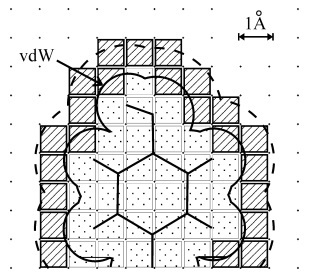
\includegraphics[width=0.5\linewidth]{figura1}}
  \caption{Representação em 2D das matrizes resultantes do segundo passo do BoGIE, as células preenchidas a tracejado diagonal correspondem à matriz de superficie, as com pontos correspondem à matriz \textit{core} e a núvem com tracejado continuo representa o corte associado à esfera de van der waals com a proteina localizada ao centro \cite{biggerPaper}.}
  \label{fig:fig2subfig}
\end{figure}

De notar, no entanto, que ambos os passos podem ser optimizados recorrendo ao GPU, no capitulo \ref{cha3} serão detalhadas possiveis abordagens à paralelização desta etapa do BiGGER, podendo trazer melhorias para além do uso do XOR.

\subsection{Geometric Hashing}
Este algoritmo é shape-explicit, ao contrário do BiGGER, que é surface-explicit - as superficies de ambos os elementos do par são quantificadas e representadas por valores binários nas superficies core e surface.

A metodologia deste método divide-se em dois passos: Pré-processamento e Reconhecimento \cite{geometry}.
A fase de pre-processamento consiste em identificar os pontos criticos na superficie do ligando e a partir destes definir frames de coordenandas locais. Sobre estes frames, serão feitas indexações com base nos pontos criticos vizinhos a um selecionado. Os indices serão usados numa hash table que contem as coordenadas locais do frame corrente (o processo é iterativo). Repete-se o procedimento para o elemento receptor. Com as coordenadas locais de ambos determinadas, procede-se para a fase de reconhecimento, em que se usa as coordenadas locais do receptor para confrontar uma correspondencia entre as coordenadas do ligando, através da hash table. Se houver demasiadas correspondencias, existe uma grande possibilidade de as curvaturas de superficie serem semelhantes, e é feita uma verificação extra com esse ambito \cite{prediction}. Na figura \ref{geometricFig}, pode-se consultar uma sintetização sobre as etapas que o método desempenha. 
A principal vantagem deste método em relação aos outros é substituir todos os passos que os algoritmos anteriores executam por uma verificação numa hash table, o que introduz rapidez em termos de computação efectuada. 

A complexidade deste método é $O(N^{3})$, sendo $N$ o número de pontos criticos a considerar. Os tempos de execução são baixos, sendo na ordem dos minutos independentemente da complexidade da previsão da docagem \cite{halperin}. No entanto a complexidade temporal é superior à do BiGGER ($O(N^{2,8})$), pelo que em teoria este último assume tempos de execução ainda menores.

\begin{figure}[ht]
  \centering
    {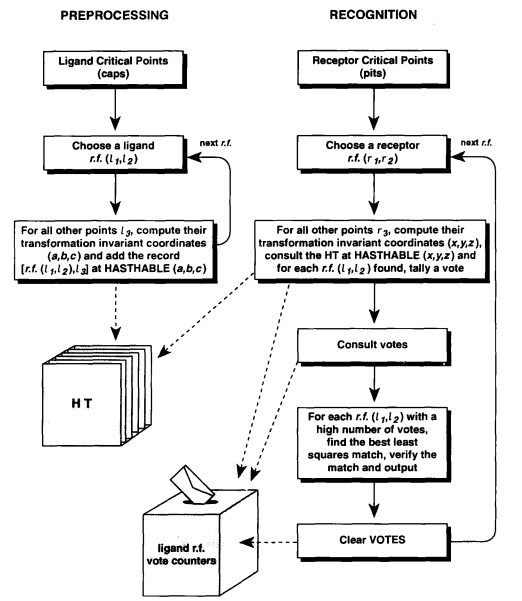
\includegraphics[width=0.5\linewidth]{geometricHashingScheme}}
  \caption{Fluxograma sobre o geometric hashing.Tirado de \cite{geometry}}
  \label{geometricFig}
\end{figure}
%duvida geometric hashing assume limitações?
%Diferenças entre o bigger e o Geometric hashing
\subsection{ZDOCK}
%amanha...

%secção GPU
\section{ O uso de GPU como ferramenta auxiliar}
\label{gpus}
GPU( \textit{Graphical Processor Unit}) consiste na unidade de processamento gráfico existente na placa gráfica instalada em qualquer computador, sendo especializada em processamento gráfico, mais precisamente renderização de gráficos 3D. 

 No entanto o GPU também é adequado para processamentos alternativos à renderização para o gaming, que são igualmente intensivos demais para o CPU. Exemplos de aplicações podem variar de cálculo financeiro até aplicações bio-informáticas, como é o caso do docking.
 
Consegue ser mais poderoso a executar instruções com custos de complexidade temporal elevado do que necessariamente o CPU, que tem um número de cores muito menor do que o GPU. \cite{nvidia2011nvidia}

 Um programador que  pretenda implementar uma paralelização para a versão sequêncial de um dado programa, recorrendo ao CPU, necessita de conhecimentos de programação com \textit{threads} assim como gerir o acesso exclusivo a variáveis partilhadas entre as mesmas, o que pode ser feito por gestão de locks ou por instruções atómicas. 
 
 O resultado consiste num programa paralelizado mas com um speedup limitado comparando com uma solução que use aceleradores no GPU.
 
  \begin{figure}[ht]
  \centering
    {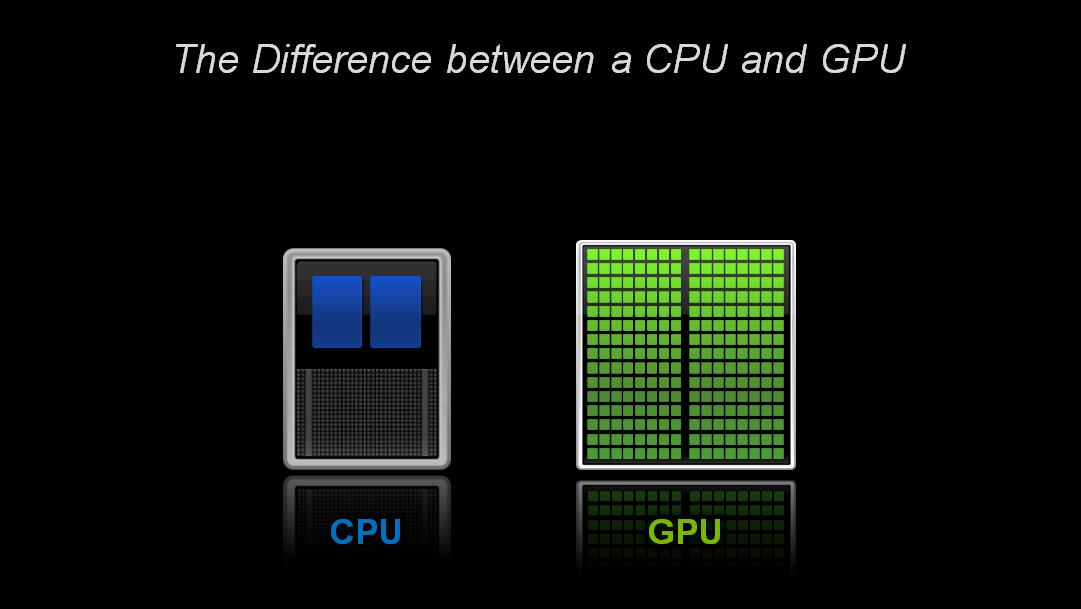
\includegraphics[width=0.5\linewidth]{cpuvsgpu}}
  \caption{Esquema ilustrativo da diferença entre o hardware do CPU e do GPU, demonstrando também a diferença de cores entre os 2. Imagem da NVIDIA}
  \label{fig:fig2subfig}
\end{figure}

\subsection{Arquitetura do GPU}

 O GPU acaba por ser uma ferramenta mais potente para paralelizar programas já que a sua arquitetura é consistente em uma quantidade variável de streamming multi-processadores (\textit{streaming multi-processors}) \cite{ritchiew}. Que por si só têm um conjunto de processadores escalares (SPs) que são também conhecidos como os cores do GPU. É possivel ter até 512 cores no total, se a arquitetura for da espécie Fermi. \cite{wittenbrink2011fermi}. Está presente ainda uma zona de memória global que pode variar entre MBs e GBs, e pode ser partilhada entre os diversos SPs.

 A arquitetura do GPU, conceptualmente, pode se dividir em duas componentes : 
 % Developers can query the compute capability by calling cudaGetDeviceProperties() and examining cudaDeviceProp.major and cudaDeviceProp.minor, or by calling the driver API function cuDeviceComputeCapability().
 
\begin{itemize}
\item \textbf{Streaming Multiprocessors} : responsáveis por executar os CUDA kernels. Funcionam como as \textit{cores} do CPU mas com caracteristicas diferentes. Têm ciclos de relógio mais baixos, mas suportam paralelismo ao nível de instrução. A evoluição dos SMs tem sido notada desde o aparecimento de hardware capaz de executar CUDA, em 2006. Em que se vão melhorando as capacidades das suas componentes: A destacar a quantidade de registos que os SMs vão dispondo, a cache L1 e o número de \textit{cores} de execução \cite{wilt_2013}.  
\item \textbf{Caches e memória}: Em que existem dois níveis de cache a considerar. As caches L1 são usadas para melhorar a latência das operações globais de escrita e leitura e como especificado no ponto anterior, estas fazem parte dos SMs. Existe ainda uma cache partilhada L2 para complementar a presença das L1. A cache L2 é uma cache de escrita/leitura com uma politica de substituição write-back . Esta cache responde a pedidos de instruções load, store assim como instruções atómicas de ambos SM e respetivas caches L1, preenchendo  de forma igual as respetivas caches \cite{nickolls2010gpu}  Os beneficios da cache L2 para o CUDA regem-se pelo aumento do armazenamento para instruções de load e store globais \cite{wittenbrink2011fermi}.  %continua...
\end{itemize}


  \begin{figure}[ht]
  \centering
    {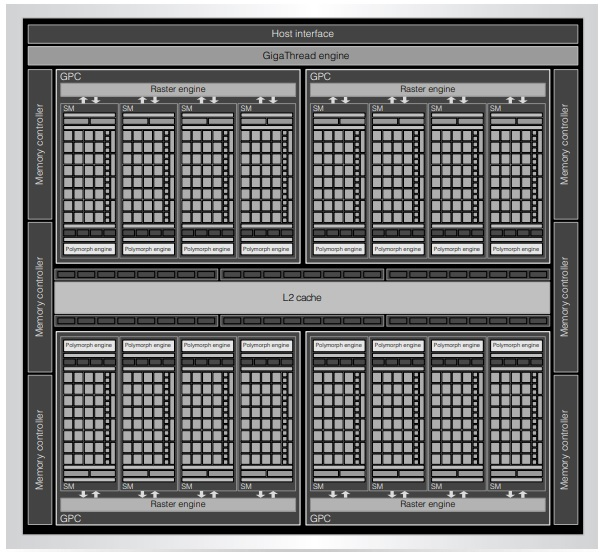
\includegraphics[width=0.5\linewidth]{fermiArch}}
  \caption{Esquema da arquitetura do GPU. Neste caso a arquitetura corresponde ao Fermi GF100. \cite{wittenbrink2011fermi}}
  \label{fig:fig2subfig}
\end{figure}

% Desenvolver o que é  um warp.
Tendo em conta a quantidade de threads individuais que têm de ser geridas e executadas em diferentes programas de forma eficiente, é empregado pelos SMs uma arquitetura especifica para o efeito, denominada SIMT (\textit{Single-Instruction Multiple-Thread}). \cite{nvidiaTesla}
Esta arquitetura permite a criação, gestão, escalonamento e execução de threads concurrentes em grupos de 32 cada. Estes grupos assumem o conceito de \textit{warps}, podendo cada bloco de threads do CUDA ter 1 ou mais warps.
\cite{gpuComputingEra}


Porém continuamos a necessitar do CPU para comunicar com o GPU, em que este último funciona como \textit{device} e o CPU funciona como \textit{host} numa interface de comunicação de dados entre os 2.
%dizer o que é que é o host e o que é que é o device.
Sendo assim é essencial usar o GPU como utensilio na paralelização de algoritmos que façam computações muito pesadas, como é o caso das etapas presentes nos algoritmos destacados nas secções anteriores.
\subsection{Modelo de programação}
\cite{optimization}
\subsection{Modelo de execução}
\cite{optimization}

\subsection{Optimizações}
De acordo com \cite{optimization}, existem três aspetos a considerar quando pretendemos optimizar um programa recorrendo a um GPU:

\begin{itemize}
\item{\textbf{Floating Point throughput}} : É dependente da percentagem de instruções de floating point incidentes. A performance aqui é optimal quando os streaming processors (SPs) estão totalmente ocupados o que é notado em aplicações com muitas threads à disposição, não precisando de muitas sincronizações entre elas, não afectando a banda larga da memoria global. O speedup do kernel pode ser melhorado neste contexto reduzindo o número de instruções que não fazem contributos para computação dos dados.

\item{\textbf{Latência de memória global}} : É possivel melhorar a latência da memória global em termos de acessos, criando um número de threads necessário para manter os SPs ocupados enquanto existem threads à espera de aceder à memória global. Este número depende da percentagem de acessos e outras instruções de grande latencia presente no programa. Quanto menor for esta percentagem, menos threads serão necessárias para atingir a ocupancia maxima dos SPs. Existe ainda outro factor que pode expor latencia de memória: O limite em registros e memória partilhada que os SMs dispõem podem impor uma limitação no número de threads que podem ser criados para esconder a latência.

\item{\textbf{Bandwidth da memória global}} : Esta variável pode limitar o throughput do sistema e aumentar a quantidade de threads não resolve o problema. Igualmente se pode referir que diminuir a carga de pressão na bandwitdh da memória global implica recorrer a mais registos e memória partilhada dos SMs para reutilização de dados, o que limita o número de threads que podem correr em simultaneo. Pelo que é necessário um balanco entre as duas medidas referidas anteriormente.
\end{itemize}

\subsection{APIs para computação acelerada}
\label {cuda}
Em termos de programação em GPUs existe como API o CUDA (\textit{Compute Unified Device Architecture}) que foi implementado pela NVIDIA 
 
 O CPU executa a parte sequêncial do programa enquanto que o GPU, com a sua quantidade numerosa de cores, executa a parte que requer computação mais intensiva como por exemplo multiplicação de matrizes (matmult), através de invocações especiais que se denominam\textit{ kernels}.\cite{nvidia2011nvidia}
  
 De notar que é necessário fazer previamente as alocações respetivas de memória do host para o device, que são feitas por parte do CPU.
   
 Um programador que queira utilizar CUDA para paralelizar o seu programa, deve transferir a toolkit respetiva ao sistema operativo em que pretende realizar o projeto, esta toolkit está disponivel na página da NVIDIA.
   
No entanto também existem mais APIs/frameworks para o efeito, como por OpenCL(\textit{Open computing language}) que é adequado para programação paralela em Free pascal enquanto que o CUDA é mais utilizado para C/C++ ou até mesmo Python (pyCUDA). 

Ambos são semelhantes no sentido de implementar o protocolo de comunicações entre o CPU e o GPU, e de permitir invocar kernels para este último computar a parte intensiva.


\section{Docking em GPU}
\label{gpus1}
Já existem vários softwares e artigos dedicados à introdução de paralelizações ao FFT \cite{ritchiew} o que muitos têm em comum é o facto de utilizarem CUDA, neste caso utilizam CuFFT. 
%Pending a correlação de matrizes é paralelizada no FFT?
O CuFFT é uma versão própria do CUDA que fornece as implementações necessárias para que a perfomance do algoritmo seja aumentada em 10x, face às versões que utilizam o CPU para o processamento respetivo\cite{nvidiaFFT} . 

\subsection {Megadock}
Um exemplo desta espécie de softwares especificos para docagem é o Megadock 4.0, este software é de origem japonesa, que melhora em relação ao Megadock 1.0 no sentido de ter implementações no ambito da computação acelerada \cite{megadock}.

Este programa é adequado para máquinas que têm muitos cores de GPU e CPU á disposição, caracteristicas tipicas de supercomputadores.

Foi implementado para GPU não só por CUDA como também por MPI (Message Passing Interface) e OpenMP. 
 O MPI, tal como a sigla expecifica, é uma API de interface de comunicação de mensagens entre processos a correr nos nós de um cluster\cite{mpiBook}. %detalhar isto, e o OpenMP
 O Megadock 4.0 é um enhancement em relação à versão 1.0 no sentido de suportar o modelo master-worker. 
O funcionamento do Megadock 4.0 envolve a criação de um processo master que faz a aquisição de uma lista de pares de proteinas e cria jobs incidentes sobre a lista para os workers.
 Estes, por sua vez, distribuem o trabalho de calcular a rotação do ligando em cada nó da lista, pelos diversos GPUs e CPUs do nó do cluster. A distribuição pelos GPUs de cada nó é feita por CUDA e pelos CPUs por OpenMP \cite{megadock40}. 
 Uma das vantagens que este protocolo assume é a tolerancia de falhas pois o nó master consegue supervisionar os resultados dos jobs executados pelos workers, além disso é escalável com o número de elementos que compõem o cluster.
 Em termos de performance e tempos de execução, os testes efectuados em 2014 (tabela \ref{tab1}) pelos autores do programa revelam a sua rapidez. O Megadock foi capaz de determinar em minutos um caso de teste que o ZDOCK determinou em duas horas.
 Os resultados referidos foram obtidos por execução no supercomputador disponível no Instituto de Tecnologia de Tóquio, TSUBAME 2.0. A dimensão amostral consiste no número total de combinações de estruturas receptoras (1936) e no mesmo número para estruturas ligandas (14400). No caso do Megadock 4.0, o valor a considerar para o tempo de cálculo ronda as 5.71h para meio milhão de jobs e 11.51H para 1 milhão de jobs. Para este último teste foi utilizado a versão 2.3 do TSUBAME\cite{megadock40}. 
 
 %Referir o que é implementado para cuda no megadock e em que medida é importante para o BIGGER
  
\begin{table}[]
\centering
\begin{tabular}{l|l|l|l|l|}
\cline{2-5}
                                             & Megadock 1.0 & Megadock 2.0 & Megadock 2.1 & ZDOCK 3.0 \\ \hline
\multicolumn{1}{|l|}{Tempo de cálculo (min)} & 13.3         & 14.7         & 16.6         & 124.6     \\ \hline
\end{tabular}
\caption{Tempos de cálculo das versões iniciais do Megadock em relação ao ZDOCK \cite{megadock}. De notar que os testes foram realizados em 2014, pelo que actualmente em 2018, pelos mesmos motivos apontados }
\label{tab1}
\end{table}

\subsection {AutoDock}
O AutoDock \cite{autoDock} consiste numa plataforma de software para auxilio na previsão da forma como pequenas moleculas, como é o caso das constituintes das drogas, se unem a receptores.
Actualmente, existem duas versões do software: AutoDock 4 e Vina. O AutoDock 4 está divido ainda em dois sub programas: autodock faz o docking do ligando com um conjunto de grelhas que fazem a descrição do complexo resultante. O segundo, autogrid, faz os calculos previos para obter as grelhas que o autodock necessita para desempenhar as suas funções.  
O AutoDock Vina é diferente do 4 no sentido de não efectuar o cálculo das grelhas de forma prévia mas sim instantaneamente. Entre as optimizações efectuadas encontra-se o uso de um método quasi-Newton BFGS
\cite{autoDockVina}
%% ====================
%% = Folder Structure =
%% ====================
%\section{Folder Structure} % (fold)
%\label{sec:folder_structure}
%
%The \novathesis\ template is organized into files and folders. At the main level it includes the following files and folders:
%
%\noindent
%\begin{tabularx}{\linewidth}{>{\ttfamily}l>{\itshape}l>{\upshape}X}
%novathesis.cls     & file    & 
%The main class file. It will include additional files from \texttt{novathesis-files} folder. 
%\\ 
%template.tex      & file    & 
%The main user file. Use this file as the main file for your thesis. 
%\\
%bibliography.bib  & file    & 
%An example of a bibliography file. You may have has many as you want. \\
%template.pdf      & file    & 
%A possible result of applying pdf\LaTeX\ to the \texttt{template.tex} file. The template supports multiple types of documents (e.g., MSc dissertation, PhD thesis, …) and multiple Schools (e.g., FCT-NOVA, FCSH-NOVA, IST-UL, FC-UL, …) and each will produce different results.
%\\
%Chapters          & folder  & Examples of thesis chapters. Replace them with your own chapters. 
%\\
%Examples          & folder  & Some more examples of the use of the template for different document types and Schools. 
%\\
%Scripts           & folder  & Some (possibly useful) scripts for Unix-based systems (Linux, Mac OSx). If you are a windows user, ignore this folder (you may safely delete it if you want). 
%\\
%novathesis-files   & folder  & 
%Additional files for the \novathesisclass\ file.  Unless you know what you are doing, avoid messing up with the files and folders inside this folder (except for deleting the unused Schools, see below). 
%\\
%\end{tabularx}
%
%The \texttt{novathesis-files} folder contains additional files and folders that complement the main \novathesisclass\ file.  These are:
%
%\noindent
%\begin{tabularx}{\linewidth}{>{\ttfamily}l>{\itshape}l>{\upshape}X}
%README.txt      & file    &
%A file that should be read!  :) 
%\\
%fix-babel.clo   & file    &
%Simple fixes to the \texttt{babel} package.
%\\
%lang-text.clo   & file    &
%Translations of important strings used in the template.  Currently fully supported are Portuguese and English, but French is on the way.  If you add translations for your own language, please be so kind and send them to me. Thank you!
%\\
%options.clo     & file    &
%Processing of \novathesisclass\ options.  \emph{Don't mess with this!}
%\\
%packages.clo    & file    &
%Additional packages to be loaded into the \novathesis\ template. \emph{You should not mess with this!}
%\\
%spine.clo       & file    &
%This file is loaded only if the option \texttt{spine=true}, and includes the typesetting of the book spine.
%\\
%ChapStyles      & folder  &
%Contains a lot of files, one for each chapter style.  If you really know what you are doing, you may add your own chapter style here.
%\\
%FontStyles      & folder  &
%Contains a few files, one for each set of fonts (main text font, chapter font, section font, subsection font, etc).  If you really know what you are doing, you may add your own set here.
%\\
%Schools         & folder  &
%Configuration files for each school.  This folder is organized into subfolders, one for each university.  \emph{You may safely delete all the subfolders except the one for your University.}  Then open the subfolder of your University and \emph{you may safely delete all the subfolders except the one for your School/Faculty}.
%\\
%\end{tabularx}
%
%As stated above, the \texttt{Schools} folder contains per-university folders and per-school (faculty) subfolders.  Currently these are the available folders:
%
%\noindent
%\begin{tabularx}{\linewidth}{>{\ttfamily}r@{~/~}>{\ttfamily}l>{\itshape}l>{\upshape}X}
%ul     & ist    & folder  & 
%The folder for the \href{http://www.tecnico.ulisboa.pt}{\emph{Instituto Superior Técnico}} of the \emph{University of Lisbon}.
%\\
%nova    & fcsh   & folder  & 
%The folder for the \href{http:www.fcsh.unl.pt}{\emph{Faculty of Human and Social Sciences}}  of the \emph{NOVA University of Lisbon}.
%\\
%nova    & fct    & folder  & 
%The folder for the \href{http:www.fct.unl.pt}{\emph{Faculty of Sciences and Technology}} of the \emph{NOVA University of Lisbon}.
%\\
%nova    & novaims    & folder  & 
%The folder for the \href{http:www.novaims.unl.pt}{\emph{Information and Management School}} of the \emph{NOVA University of Lisbon}.
%\\
%\end{tabularx}

%% section folder_structure (end)
%
%% ===================
%% = Package options =
%% ===================
%\section{\novathesisclass\ Class Options} % (fold)
%\label{sec:package_options}
%
%The \novathesis\ class can be customized with the options listed below.
%
%\newcommand{\classoption}[3]{\textbf{#1=OPT}\qquad #2\\\qquad\emph{#3}\\}
%
%\noindent
%\begin{ctabular}{@{}p{\linewidth}@{}}
%  \toprule
%  \classoption{docdegree}%
%    {phd(*), phdplan, phdprop, msc, mscplan, bsc}%
%    {The type of the document: PhD Thesis (default), PhD Plan, PhD Proposal, MSc Disseration, MSc Plan, BSc Report}
%    \midrule
%  \classoption{school}%
%		{nova/fct(*), nova/fcsh, nova/ims, ul/ist, ul/fc}%
%    {The name of the school. This option changes the typesetting of the cover and some School specific formating, like margins, fonts, paragraph spacing and indentation, etc…}
%    \midrule
%  \classoption{lang}%
%    {en(*), pt}%
%    {The main language for the document.  Currently only Portuguese and English are supported.  Other languages are expected to be support in forthcoming versions.}
%    \midrule
%  \classoption{fontstyle}%
%    {bookman, charter, fourier, kpfonts(*), mathpazo1, mathpazo2, newcent}%
%    {The font set to be used in the document.  Please note that a font set include definitions for the main text, headings, maths, etc.}
%    \midrule
%  \classoption{chapstyle}%
%    {bianchi, bluebox, brotherton, dash, default, elegant(*), ell, ger, hansen, ist, jenor, lyhne, madsen, pedersen, veelo, vz14, vz34, vz43}%
%    {The chapter style, i.e., the look of the chapter beginning.}
%    \midrule
%  \classoption{converlang}%
%    {en, pt(*)}%
%    {The language to be used when typesetting the cover page.}
%    \midrule
%  \classoption{otherlistsat}%
%    {front(*), back}%
%    {Where to put the other lists besides the table of contents. The default is (\texttt{front}) before the main text.  But some scientific areas prefer them at the end of the document (\texttt{back}), just before the Appendixes.}
%    \midrule
%  \classoption{aftercover}%
%    {true, false(*)}%
%    {Include or don't include the contents of the “\texttt{aftercover}” file. The default is for this file to be ignored (if if it exists).}
%    \midrule
%  \classoption{linkscolor}%
%    {darkblue(*), black}%
%    {The color for all the hyperlinks in the PDF file.  The “\texttt{media=paper}” option (see below) will override this option to “\texttt{black}”}
%    \midrule
%  \classoption{spine}%
%    {true, false(*)}%
%    {Generate the book spine and the last page in the PDF.}
%    \midrule
%  \classoption{biblatex}%
%    {OPT=\{list of options for \texttt{biblatex}\}}%
%    {Customize \texttt{biblatex}, the bibliography management system used in this class. Probably you will want to change the value of the \texttt{biblatex} “\texttt{style}” option. For other customizations of \texttt{biblatex} check its manual.}
%    \midrule
%  \classoption{memoir}%
%    {OPT=\{list of options for \texttt{memoir}\}}%
%    {Customize the base class \texttt{memoir}. The \texttt{memoir} manual should be the first document to be consulted when looking for “\textbf{how can I do this?}” You may wnat to change the base font size from 11pt to a smaller (10pt) or larger (12pt) size.  Also, remember to change the “\texttt{draft}” to final when your document is finished.}
%    \midrule
%  \classoption{media}%
%    {screen(*), paper}%
%    {Behavior to be customized in the school options/configuration. Expected definitions for screen are: left and right margins are equal and use colored links. Expected definitions for paper are: left and right margins are different and use black links.}
%    \bottomrule
%\end{ctabular}
%
%\section{Additional considerations about the class options} % (fold)
%\label{sec:additional_considerations}
%
%In this section we will provide some additional considerations about some of the customizations available as class options.
%
%\subsection{The main language} % (fold)
%\label{sub:the_main_language}
%
%The choice of the main language with the option “\texttt{lang=OPT}” affects:
%
%\begin{itemize}
%	\item \textbf{The order of the summaries.} First is printed the abstract in the main language and then in the foreign language. This means that if your main language for the document in English, you will see first the “abstract” (in English) and then the “resumo” (in Portuguese). If you switch the main language for the document for Portuguese, it will also automatically switch the order of the summaries to “resumo” and then “abstract”.
%	\item \textbf{The names for document sectioning.} E.g., ``Chapter'' vs.\ ``Capítulo'', ``Table of Contents'' vs.\ ``Índice'', ``Figure'' vs.\ ``Figura'', etc.
%	\item \textbf{The type of documents in the bibliogrpahy.} E.g., ``Technical Report'' vs.\ ``Relatório Técnico'', ``PhD Thesis'' vs.\ ``Tese de Doutoramento'', etc.
%\end{itemize} 
%
%No mater which language you chose, you will always have the appropriate hyphenation rules according to the language at that point. You always get Portuguese hyphenation rules in the ``Resumo'', english hyphenation rules in the ``Abstract'', and then the main language hyphenation rules for the rest of the document.
%
%% subsection the_main_language (end).
%
%% section additional_consideration (end)
%
%
%\subsection{Class of Text} % (fold)
%\label{sub:class_of_text}
%
%You must choose the class of text for the document. The available options are:
%
%\begin{enumerate}
%	\item \textbf{bsc} --- BSc graduation report.
%	\item \textbf{*mscplan} --- Preparation of MSc dissertation. This is a preliminary report graduate students at DI-FCT-NOVA must prepare to conclude the first semester of the two-semesters MSc work. The files specified by \verb!\dedicatoryfile! and \verb!\acknowledgmentsfile! are ignored, even if present, for this class of document.
%	\item \textbf{msc} --- MSc dissertation.
%	\item \textbf{phdprop} ---  Proposal for a PhD work. The files specified by \verb!\dedicatoryfile! and \verb!\acknowledgmentsfile! are ignored, even if present, for this class of document.
%	\item \textbf{prepphd} ---  Preparation of a PhD thesis. This is a preliminary report PhD students at DI-FCT-NOVA must prepare before the end of the third semester of PhD work. The files specified by \verb!\dedicatoryfile! and \verb!\acknowledgmentsfile! are ignored, even if present, for this class of document.
%	\item \textbf{phd} --- PhD dissertation.
%\end{enumerate}
%% subsection class_of_text (end)
%
%% ============
%% = Printing =
%% ============
%\subsection{Printing} % (fold)
%\label{sub:printing}
%
%You must choose how your document will be printed. The available options are:
%\begin{enumerate}
%	\item \textbf{oneside} --- Single side page printing.
%	\item \textbf{*twoside} --- Double sided page printing.
%\end{enumerate}
%% subsection printing (end)
%
%% =============
%% = Font Size =
%% =============
%\subsection{Font Size} % (fold)
%\label{ssec:font_size}
%
%You must select the encoding for your text. The available options are:
%\begin{enumerate}
%	\item \textbf{11pt} --- Eleven (11) points font size.
%	\item \textbf{*12pt} --- Twelve (12) points font size. You should really stick to 12pt\ldots
%\end{enumerate}
%% subsection font_size (end)
%
%% =================
%% = Text encoding =
%% =================
%\subsection{Text Encoding} % (fold)
%\label{ssec:text_encoding}
%
%You must choose the font size for your document. The available options are:
%\begin{enumerate}
%	\item \textbf{latin1} --- Use Latin-1 (\href{http://en.wikipedia.org/wiki/ISO/IEC_8859-1}{ISO 8859-1}) encoding.  Most probably you should use this option if you use Windows;
%	\item \textbf{utf8} --- Use \href{http://en.wikipedia.org/wiki/UTF-8}{UTF8} encoding.    Most probably you should use this option if you are not using Windows.
%\end{enumerate}
% subsection font_size (end)

% ============
% = Examples =
% ============
%\subsection{Examples} % (fold)
%\label{ssec:examples}
%
%Let's have a look at a couple of examples:
%
%\begin{itemize}
%	\item Preparation of PhD thesis, in portuguese, with 11pt size and to be printed single sided (I wonder why one would do this!)\\
%	\verb!\documentclass[prepphd,pt,11pt,oneside,latin1]{thesisdifct-nova}!
%	\item MSc dissertation, in english, with 12pt size and to be printed double sided\\
%	\verb!\documentclass[msc,en,12pt,twoside,utf8]{thesisdifct-nova}!
%\end{itemize}
%% subsection examples (end)
%
%\section{How to Write Using \LaTeX} % (fold)
%\label{sec:how_to_write_using_latex}
%
%Please have a look at Chapter~\ref{cha:a_short_latex_tutorial_with_examples}, where you may find many examples of \LaTeX constructs, such as Sectioning, inserting Figures and Tables, writing Equations, Theorems and algorithms, exhibit code listings, etc.
%
%% section how_to_write_using_latex (end)
%
%
%
%\section{Exmaple glossary and acronyms}
%%
%% \todo[inline]{A a note in a line by itself.}
%%
%This is the first occurrence of an abbreviation: \gls{abbrev}. And now the second occurrence of the same abbreviation: \gls{abbrev}. And a new acronym with capital letter: \Gls{xpt} and reused \gls{xpt}.  Let's also use a few other acronyms such as \gls{aaa}, \gls{aab}, \gls{aba}, \gls{bbb} and \gls{xpt}.
%
%
%Lets add the term ``\gls{computer}'' to the glossary!
%
% Please note that
% \begin{center}
%   \textbf{\large this package and template are not official for FCT/NOVA}.
% \end{center}
